\documentclass[a4paper]{article}

\usepackage[romanian]{babel}
\usepackage{amsmath}
\usepackage{indentfirst} % indenteaza primul paragraf din fiecare sectiune
\usepackage{graphicx}
\usepackage{hyperref}
\usepackage{caption}
\usepackage{subcaption} % pentru subfiguri

\title{Referat: Determinarea constantei lui Planck din studiul efectului
fotoelectric}
\author{Nicolas Dumitru}
\date{}

\begin{document}

\maketitle

\section{Scopul lucrării}
În această lucrare se studiază efectul fotoelectric extern produs pe catodul
unei celule fotoelectrice, se măsoară energia cinetică a electronilor ca funcție
de frecvența luminii incidente pe catod și constanta Planck $h$, arătându-se că
energia cinetică a electronilor este independentă de intensitatea luminii
incidente.

\section{Teoria lucrării}

Electronii pot fi emiși de către suprafața anumitor metale prin iradierea
acestora cu lumină având lungimi de undă mici (efect fotoelectric). Energia
electronilor emiși depinde de frecvența $\nu_0$ a luminii incidente, nu și de
intensitatea acesteia. Intensitatea fasciculului de lumină incident determină
doar \underline{numărul} de electroni liberi emiși.

Aceste rezultate experimentale contrazic principiile fizicii clasice și au fost
interpretate pentru prima dată de către Albert Einstein în 1905. Acesta a
postulat că lumina este un flux de particule (fotoni) și că energia unui foton
este proporțională cu frecvența luminii:

\begin{equation}
	E = h \nu
\end{equation}
unde $h$ este constanta lui Planck.

Ecuația de conservare a energiei in procesul de emisie a fotoelectronilor este:
\begin{equation}
	E_c = h \nu - L_{extr}
\end{equation}
unde $E_c$ e energia cinetică a fotonului emis, iar $L_{extr}$ e lucrul mecanic
de extracție a electronilor din metal.

Putem determina constanta lui Planck din punct de vedere experimental prin
expunerea unei celule fotoelectrice la lumină monocromatică (lumină ce are o
singură lungime de undă, spre deosebire de fasciculele luminoase obișnuite,
nefiltrate, care prezintă un amestec de lungimi de unda) și măsurarea energiei
cinetice a fotoelectronilor emiși.

În figura \ref{fig:catod} este prezentată schema experimentului, în care fasciculul de lumină
este incident pe catodul dispozitivului (în cazul nostru acesta este un fir de
platină plasat pe o suprafață de potasiu).

O parte dintre electronii emiși ajung la anod, unde formează curentul
fotoelectric prin circuit. În cazul în care se aplică un potențial negativ care
este crescut treptat asupra fotoelectronilor emiși de către catod, va rezulta o
descreștere a fotocurentului până la anularea sa.

Tensiunea aplicată, la care acesta se anulează poartă numele de tenisiune de
stopare $U_0$.

Atunci când tensiunea negativă aplicată anodului atinge valoarea XXX, chiar și
electronii cu cea mai mare energie cinetică și cel mai mic lucru mecanic de
extracție din catod nu mai pot ajunge la anod.

În cadrul experimentului, tensiunea aplicată pe anod este generată cu ajutorul
unui condensator care este încărcat de către electronii incidenți până la
tensiunea $U$ (așa cum se arată în figura 1).

Putem calcula astfel energia cinetică a electronilor cu ajutorul ecuației de
conservare a energiei, în cazul în care măsurăm tensiunea $U_0$.
\begin{equation}
	e U_0 = h \nu - L_{extr}
\end{equation}

Observăm că atunci când reprezentăm tensiunea de stopare $U_0$ ca o funcție de
frecvență, ecuația anterioară reprezintă ecuația unei drepte cu panta:
\begin{equation}
	m = \frac{\Delta U_0}{\Delta \nu} = \frac{h}{e}
\end{equation}

Atunci când cunoaștem sarcina elementară a electronului $e$, ecuatia anterioară
poate fi folosită pentru a afla constanta lui Planck.

\section{Schițe}
\begin{figure}[htbp]
	\centering
	\begin{subfigure}{0.45\textwidth}
		\centering
		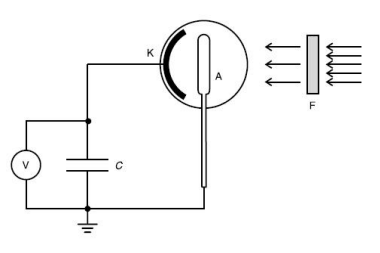
\includegraphics[width=\linewidth]{catod.png}
		\caption{Catodul}
		\label{fig:catod}
	\end{subfigure}
	\hfill
	\begin{subfigure}{0.45\textwidth}
		\centering
		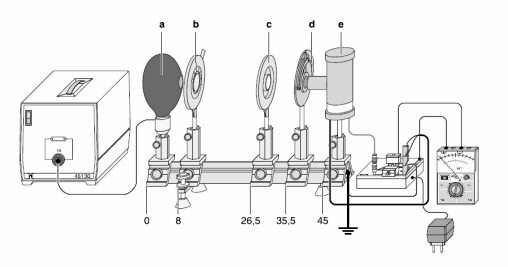
\includegraphics[width=\linewidth]{device.png}
		\caption{Dispozitivul experimental}
		\label{fig:device}
	\end{subfigure}
	\caption{}
\end{figure}

\end{document}
